\begin{tikzpicture}

\node[anchor=south west,inner sep=0] (IMG) at (0,0) {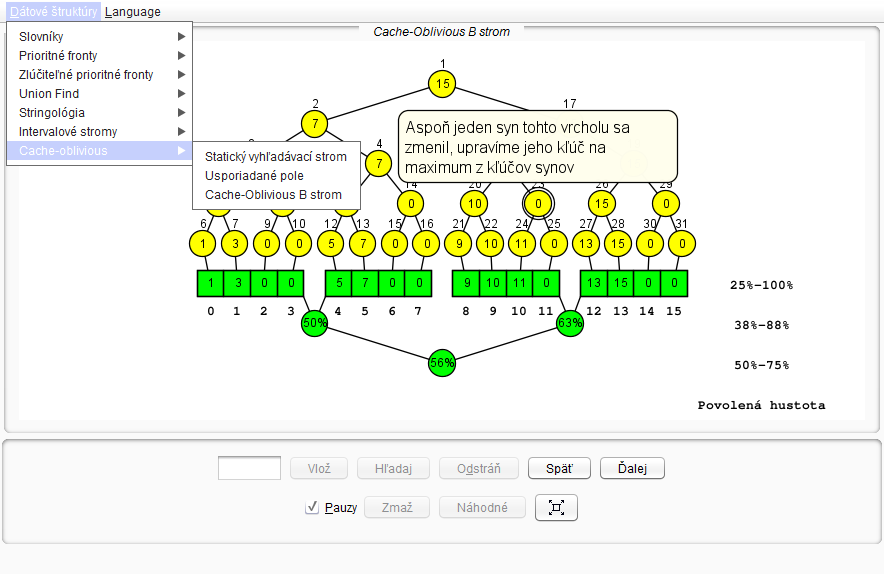
\includegraphics[width=18cm]{\FiguresPath/screenshots/bmp_cobtree_menu_sk}};
\draw [thick, darkgray] (IMG.south west) rectangle (IMG.north east);

%\draw[draw=red,xstep=1,ystep=1] (0,0) grid (18,12);
%\foreach \x in {0,1,...,18} { \node [anchor=north] at (\x,0) {\x}; }
%\foreach \y in {0,1,...,12} { \node [anchor=east] at (0,\y) {\y}; }

\draw [thick, ->] (2, 12.5) node [anchor=west] {Výber dátovej štruktúry} to [in=90, out=180] (1, 11.75);
\draw [thick, ->] (3, 12) node [anchor=west] {Výber jazyka} to [in=90, out=180] (2.5, 11.75);

\draw [thick, ->] (10, 12.5) node [anchor=west] {Aktuálna dátová štruktúra} to [in=90, out=180] (9, 11.25);

\draw [thick, ->] (13, 12) node [anchor=west] {Popis vykonávanej akcie} to [in=90, out=180] (11, 9.5);

\draw [thick, decoration={brace, amplitude=10pt, 
	/tikz/postaction = {
		decoration = {
			markings,
			mark = at position 0.5 with \coordinate (CP);
		}, decorate
	}
}, decorate] (4.25, 1) -- (4.25, 2.5);
\draw [thick] (2.5, -0.5) node [anchor=east] {Ovládací panel} to [in=180, out=0](CP);

\draw [thick, ->] (7, -0.5) node [anchor=west] {Povolenie krokovania} to [in=270, out=180] (6.35, 1.15);

\draw [thick, decoration={brace, amplitude=10pt, mirror,
	/tikz/postaction = {
		decoration = {
			markings,
			mark = at position 0.5 with \coordinate (PN);
		}, decorate
	}
}, decorate] (10.65, 1.95) -- (13.7, 1.95);
\draw [thick] (13, -0.5) node [anchor=west] {Krokovanie dopredu / dozadu} to [in=270, out=180] (PN);

\end{tikzpicture}